\chapter{Conclusion}

\begin{table}[]
\centering
\caption{Results}
\label{resultAll}
\begin{tabular}{ll}
Tf-IDF   & 0.44±0.04 \\
PVDM(dbow) & 0.40    \\
FastText &  ~0.51   \\
FastText(Pinyin) &  ~0.51  \\
Simaese-CBOW & 0.41 (± 0.04)
\end{tabular}
\end{table}

\begin{table}[]
\centering
\caption{FastText}
\label{fasttext}
\begin{tabular}{llllll}
   & 8 & 12 & 16 & 32 & 64 \\
no segmentation  & 0.369 & 0.375 & 0.389 & 0.372 & 0.368 \\
segmentation  & 0.515 & 0.515 & 0.514 & 0.516 & 0.513 \\
segmentation + pinyin  & 0.513 & 0.518 & 0.516 & 0.517 & 0.51 \\
\end{tabular}
\end{table}

\begin{table}[]
\centering
\caption{ResultsDoc2Vec}
\label{resultAll}
\begin{tabular}{lll}
      & Test set & Training Set \\
dm/c  & 0.384 &  0.384 \\
dbow &  0.404  & 0.457 \\
dm/m &  0.38  & 0.436
\end{tabular}
\end{table}


\section{Experiment Settings}


We used baseline TD-IDF plus SVM with linear kernel as baseline. Since the original distribution for classes is a little skewed, most the test sample is classified into 2 major classes.
We compared it with other models with different settings. \\

For PVDB, we use 3 different models dm/c and dm/m and dbow. All of them, we choose most commonly-used parameters,dm : dimension:100, window size:10, negative:5, hs:0 and we tested both dm with concatenation of context vectors (dm/c) and average of context vectors(dm/m). The other model dbow, we chose the same parameters.

In FastText experiment, we iterated through the parameters like window size from 8 to 100, loss function ns,hs,softmax.  Since the result did't indicate significant difference between these parameters, we only display 1 of them as reference.

Additionally, we also tried to convert data set to pinyin to evaluate if the pinyin improve the sematic recognition for FastText ,which support vocabulary expansion with subword information \cite{bojanowski2016enriching}. 

\begin{figure}[h]
    \centering
	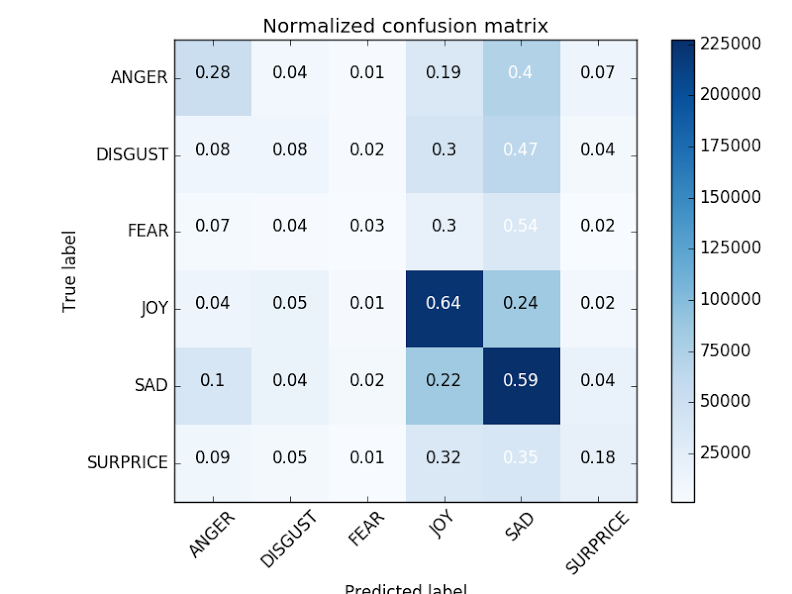
\includegraphics[width=.9\linewidth]{tf-idf}
    \caption{The confusion matrix for TF-IDF+ SVM}
    \label{fig:sub1}
\end{figure}

\begin{figure}[h]
    \centering
	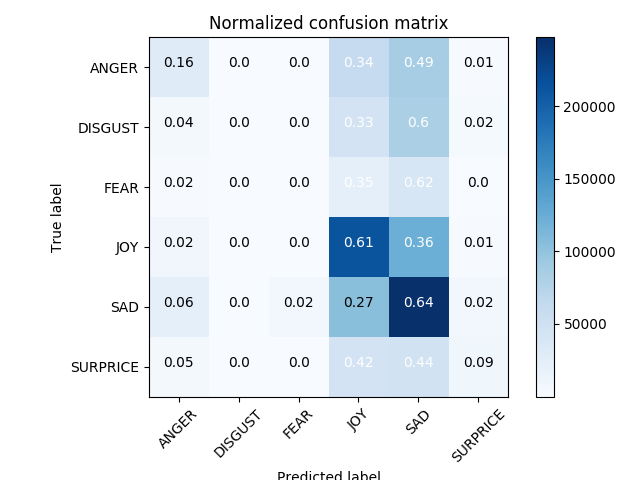
\includegraphics[width=.9\linewidth]{sc-ratio}
    \caption{The confusion matrix for two models comparison}
    \label{fig:sub2}
\end{figure}